%!TEX TS-program = xelatex
%!TEX encoding = UTF-8 Unicode

\documentclass[12pt]{extarticle}
% extarticle is like article but can handle 8pt, 9pt, 10pt, 11pt, 12pt, 14pt, 17pt, and 20pt text

\def \ititle {Origins of Mind}
 
\def \isubtitle {Lecture 02}
 
\def \iauthor {Stephen A. Butterfill}
\def \iemail{s.butterfill@warwick.ac.uk}
\date{}

%for strikethrough
\usepackage[normalem]{ulem}

\input{$HOME/Documents/submissions/preamble_steve_handout}

%\bibpunct{}{}{,}{s}{}{,}  %use superscript TICS style bib
%remove hanging indent for TICS style bib
%TODO doesnt work
\setlength{\bibhang}{0em}
%\setlength{\bibsep}{0.5em}


%itemize bullet should be dash
\renewcommand{\labelitemi}{$-$}

\begin{document}

\begin{multicols}{3}

\setlength\footnotesep{1em}


\bibliographystyle{newapa} %apalike

%\maketitle
%\tableofcontents




%--------------- 
%--- start paste



\def \ititle {Origins of Mind}
 
\def \isubtitle {Lecture 02}
 
 
 
\
 
 
 
\begin{center}
 
{\Large
 
\textbf{\ititle}: \isubtitle
 
}
 
 
 
\iemail %
 
\end{center}
 
 
 
\section{Objects vs Features}
 
Knowledge of objects depends on abilities to (i) segment objects, (ii) represent them as 
persisting and (iii) track their interactions.
 
The question for this lecture is,
How do humans come to meet the three requirements on knowledge of objects?
 
 
 
\section{Segmentation and the Principles of Object Perception}
 
`infants perceive the boundaries of a partly hidden object by analyzing the movements of 
its surfaces: infants perceived a connected object when its ends moved in a common 
translation behind the occluder. Infants do not appear to perceive a connected object 
by analyzing the colors and forms of surfaces: they did not perceive a connected object 
when its visible parts were stationary, its color was homogeneous, its edges were aligned, 
and its shape was simple and regular'  \citep{kellman:1983_perception}.
 
\textbf{Principles of Object Perception \citep{Spelke:1990jn}}
 
cohesion—‘two surface points lie on the same object only if the points are linked by a path of 
connected surface points’
 
boundedness—‘two surface points lie on distinct objects only if no path of connected surface points 
links them’
 
rigidity—‘objects are interpreted as moving rigidly if such an interpretation exists’
 
no action at a distance—‘separated objects are interpreted as moving independently of one another if such an 
interpretation exists’
 
 
What is the status of these principles?
 
\begin{enumerate}

\item We (as perceivers) start with a cross-modal representation of three-dimensional 
perceptual features which includes their locations and trajectories.

\item Our task is to get from these representations of features to representations of objects.

\item \emph{Descriptive component} We do this as if in accordance with certain principles 
(cohesion, boundedness, rigidity, and no action at a distance).

\item \emph{Explanatory component}  We acquire representations of objects because we apply the 
principles to representations of features and draw appropriate inferences.

\end{enumerate}

Three Questions: 
1. How do four-month-old infants model physical objects?
2. What is the relation between the model and the infants?
3. What is the relation between the model and the things modelled (physical objects)?

 
‘Chomsky’s nativism is primarily a thesis about knowledge and belief; it aligns problems 
in the theory of language with those in the theory of knowledge.  Indeed, as often as not, 
the vocabulary in which Chomsky frames linguistic issues is explicitly epistemological.  
Thus, the grammar of a language specifies what its speaker/hearers have to know qua speakers 
and hearers; and the goal of the child’s language acquisition process is to construct a 
theory of the language that correctly expresses this grammatical knowledge.’
\citep[p.\ 11]{Fodor:2000cj}
 
\textbf{The simple view}
The principles of object perception are things that we know or believe, 
and we generate expectations from these principles by a process of inference.
 
‘objects are conceived: Humans come to know about an object’s unity, boundaries, and 
persistence in ways like those by which we come to know about its material composition or its 
market value’
\citep[p.\ 198]{Spelke:1988xc}.
 
 
 
\section{Permanence}
 
\textit{Object permanence}:
the ability to know things about, or represent, objects you aren't currently perceiving.
 
\emph{Principle of continuity}  An object traces exactly one connected path over space and time \citep[p.\ 113]{spelke:1995_spatiotemporal}.
 
\begin{center}
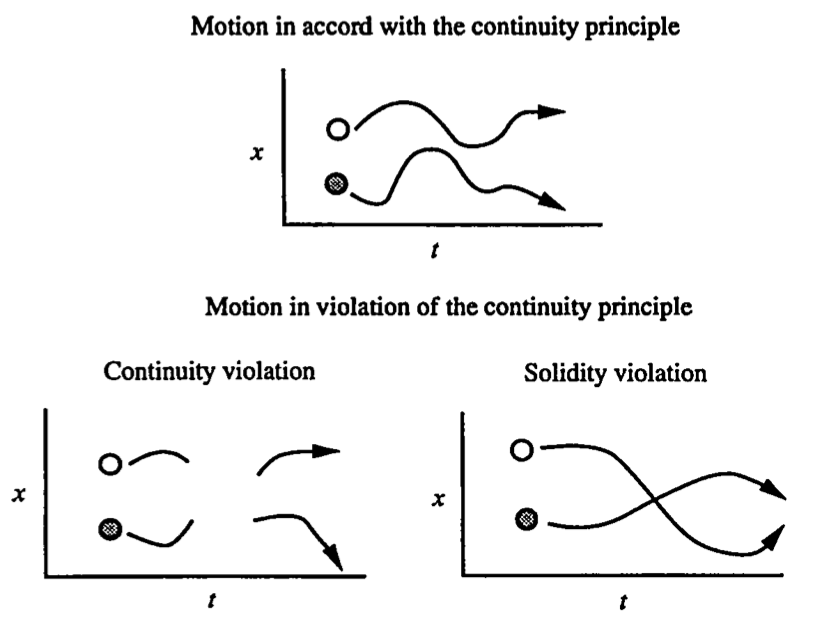
\includegraphics[scale=0.3]{img/spelke_1995_fig1.neg.png}
\end{center}
 
Interpreting violation-of-expectation experiments:
 
‘evidence that infants look reliably longer at the unexpected than at the expected event is taken to indicate that they (1) possess the expectation under investigation; (2) detect the violation in the unexpected event; and (3) are surprised by this violation. The term surprise is used here simply as a short-hand descriptor, to denote a state of heightened attention or interest caused by an expectation violation.’
\citep[p.\ 168]{wang:2004_young}
 
‘To make sense of such results [i.e. the results from violation-of-expectation tasks], we … must assume that infants, like older learners, formulate … hypotheses about physical events and revise and elaborate these hypotheses in light of additional input.’
\citep[p.\ 329]{Aguiar:2002ob}
 
Object permanence is found in nonhuman animals including
 
\begin{enumerate}
 
\item monkeys \citep{santos:2006_cotton-top}
 
\item lemurs \citep{deppe:2009_object}
 
\item crows \citep{hoffmann:2011_ontogeny}
 
\item dogs and wolves \citep{fiset:2013_object}
 
\item cats \citep{triana:1981_object}
 
\item chicks \citep{chiandetti:2011_chicks_op}
 
\item dolphins \citep{jaakkola:2010_what}
 
\item ...
 
\end{enumerate}
 
 
 
\section{Causal Interactions}
 
‘object perception reflects basic constraints on the motions of physical bodies …’
\citep[p.\ 51]{Spelke:1990jn}
 
‘A single system of knowledge … appears to underlie object perception and physical reasoning’
\citep[p.\ 175]{Carey:1994bh}
 
 
 
\section{Recap and Questions}
 
\emph{Question 1}  How do humans come to meet the three requirements on knowledge of objects?
 
\emph{Discovery 1} Infants manfiest all three abilities from around four months of age or earlier.
 
\emph{Discovery 2} Although abilities to segment objects, to represent them as persisting through occlusion and  to track their causal interactions are conceptually distinct, they may all be consequences of a single mechanism (in humans and perhaps in other animals).
 
\emph{Question 2} What is the relation between the principles of object perception and infants’ looking behaviours?
 
The \emph{simple view} is the view that the principles of object perception are things that we know, and we generate expectations from these principles by a process of inference.
 
 
 
\section{A Problem}
 
‘action demands are not the only cause of failures on occlusion tasks’
\citep[p.\ 291]{shinskey:2012_disappearing}
 
‘A similar permanent dissociation in understanding object support relations  
might exist in chimpanzees. They identify impossible support relations in looking tasks, 
but fail to do so in active problem solving.’
\citep{gomez:2005_species}
 
‘to date, adult primates’ failures on search tasks appear to 
exactly mirror the cases in which human toddlers perform poorly.’
\citep[p.\ 17]{santos:2009_object}
 
 
 
\section{Like Knowledge and Like Not Knowledge}
 
‘no concept causes more problems in discussions of infant cognition than that of representation’
\citep{Haith:1998aq}.
 
  

%--- end paste
%--------------- 
 
\footnotesize 
\bibliography{$HOME/endnote/phd_biblio}

\end{multicols}

\end{document}